\documentclass[12pt,oneside]{fithesis2}
\usepackage{graphicx}
\usepackage[english]{babel}       % Multilingual support
\usepackage[utf8]{inputenc}       % UTF-8 encoding
\usepackage[T1]{fontenc}          % T1 font encoding
\usepackage[                      % A sans serif font that blends well with Palatino
  scaled=0.86
]{berasans}
\usepackage[                      % A tt font if you do not like LM's tt
  scaled=1.03
]{inconsolata}
\usepackage{blindtext}
\usepackage[hyphens]{url}
\usepackage[                      % Clickable links
  plainpages = false,               % We have multiple page numberings
  pdfpagelabels,
  hidelinks                     % Generate pdf page labels
]{hyperref}            % Lorem ipsum generator
\usepackage{listings}
\usepackage[svgnames]{xcolor}

\usepackage{amsthm}
\newtheorem{definition}{Definition}

\usepackage{ftnxtra}
\usepackage{fnpos}

\definecolor{javared}{rgb}{0.6,0,0} % for strings
\definecolor{javagreen}{rgb}{0.25,0.5,0.35} % comments
\definecolor{javapurple}{rgb}{0.5,0,0.35} % keywords
\definecolor{javadocblue}{rgb}{0.25,0.35,0.75} % javadoc
\definecolor{maroon}{rgb}{0.5,0,0}
\definecolor{darkgreen}{rgb}{0,0.5,0}

\lstdefinestyle{eclipse_java}
{
	language=Java,
	basicstyle=\ttfamily\footnotesize,
	keywordstyle=\color{javapurple}\bfseries,
	stringstyle=\color{javared},
	commentstyle=\color{javagreen},
	morecomment=[s][\color{javadocblue}]{/**}{*/},
	tabsize=2,
	showspaces=false,
	showstringspaces=false
}


\lstdefinestyle{my_xml}
{
	language=XML,
	basicstyle=\ttfamily,
	morestring=[s]{"}{"},
	morecomment=[s]{?}{?},
	morecomment=[s]{!--}{--},
	commentstyle=\color{darkgreen},
	moredelim=[s][\color{black}]{>}{<},
	moredelim=[s][\color{red}]{\ }{=},
	stringstyle=\color{blue},
	identifierstyle=\color{maroon},
	tabsize=2,
	showstringspaces=false
}

\lstdefinestyle{json}
{
	basicstyle=\ttfamily,
	tabsize=2,
	showstringspaces=false,
	keywordstyle=\bfseries,
	morekeywords={thrown}
}

\lstdefinestyle{byteman}
{
	tabsize=2,
	showstringspaces=false,
	basicstyle=\ttfamily,
}

\lstset{frame=lrtb, captionpos=b, breaklines=true, showstringspaces=false, basicstyle=\ttfamily}
\lstset{language=Java}
\lstset{language=XML}

\usepackage[chapter]{minted}

\usepackage{multicol}
\usepackage{enumitem}
\usepackage{nameref}

\thesislang{en}                   % The language of the thesis
\thesistitle{Monitoring Extension for Microservices Platform SilverWare}       % The title of the thesis
\thesissubtitle{Diploma Thesis}  % The type of the thesis
\thesisstudent{Bc. Jaroslav Dufek}          % Your name
\thesiswoman{false}                % Your gender
\thesisfaculty{fi}                % Your faculty
\thesisyear{\the\year}     % The academic term of your thesis defense
\thesisadvisor{Mgr. Martin Večeřa}   % Your advisor

\begin{document}
\sloppy

  \FrontMatter                    % The front matter
    \ThesisTitlePage                % The title page
    \begin{ThesisDeclaration}       % The declaration
      \DeclarationText
      \AdvisorName
    \end{ThesisDeclaration}
    \begin{ThesisThanks}            % The acknowledgements (optional)
      Foremost I would like to thank my family, mom, dad, grandmother and grandfather and my sister, who all generously supported me throughout my whole study, even if it's been hard with me sometimes. Also I would like to thank my uncle Zdenek for introducing me to programming, which became my hobby and because of it I chose to study this field of knowledge. Then I would like to thank my thesis advisor Martin Večeřa for having a meeting with me and helping me whenever I needed. And lastly my good friend Radek Koubský, who also helped me a few times with understanding the SilverWare platform.
    \end{ThesisThanks}
    \begin{ThesisAbstract}          % The abstract
This thesis introduces the microservice architecture, its benefits and drawbacks and how it differs from the common monolithic architecture, followed by quick presentation of SilverWare microservice platform.

Consequently it presents the basics of monitoring microservices and some of the most popular open-source monitoring tools, followed by my implementation of monitoring extension for SilverWare platform.
    \end{ThesisAbstract}
    \begin{ThesisKeyWords}          % The keywords
       Microservice architecture, monitoring, containers, Docker, SilverWare OpenTracing, Metrics, Graphite, Zipkin 
    \end{ThesisKeyWords}
    \tableofcontents                % The table of contents
%   \listoftables                   % The list of tables (optional)
%   \listoffigures                  % The list of figures (optional)
  
  \MainMatter                     % The main matter
\chapter{Introduction}

\section{Goals and challenges}

My overall goal was to explore very young realm of services and applications written as microservices with focus on monitoring such systems and consequently implement a monitoring provider extension for one of the microservice frameworks called SilverWare.

Because this field was completely new to me, I first needed to read some introduction books to even get a grasp of what microservices are, why is everyone so excited about them, what are their core principles, what can they offer and what challenges they come with.

Afterwards I learned basics of using containers in applications with focus on OpenShift/Kubernetes/Docker platform, which provide a fitting environment for microservice applications and are very often mentioned in various articles. Then I briefly tried out contemporary microservice frameworks and platforms and finally got my hands on SilverWare which code and internal workings I needed to study thoroughly so I could develop a suitable extension for it.

When I had sufficient general insight into the microservices landscape I steered my attention towards actual monitoring issues of microservices and looked for appropriate standards and solutions which I could integrate into the SilverWare microservice framework.

\section{Structure of the Thesis}

In the beginning I will introduce the microservice architecture, its key principles, how it is different to traditional monolithic architecture, its benefits and drawbacks and when it is good to utilize it.

Follows a brief explanation of microservices relation to containers, introduction of microservice framework SilverWare and closer look at some of its most important components.

Afterwards we explore the monitoring aspect of microservices, why it is important, different areas of monitoring and lastly we go through some of the open-source solutions for monitoring.

Then I will present my monitoring extension for SilverWare in form of two new microservice providers for tracing and metrics, their capabilities and examples of their usage.

In the end I will showcase a quickstart application that uses miscellaneous modules of SilverWare to create a interesting application which reports monitoring data to chosen monitoring tools.

\chapter{Microservices}

For many years now, we have been finding better ways to build systems. We have been learning from what has come before, adopting new technologies, and observing how a new wave of technology companies operate in different ways to create IT systems that help make both their customers and their own developers happier. \cite{ma}

Software systems have become more and more complex as their scale increased. Scale in the form of scope, volume, and user interactions. This increase of scale has brought many problems upon traditional way of developing enterprise applications. Problems such as increased complexity of the software and so increased development time, tight coupling of system parts and so inability to change, increased deployment dependencies and deployment time. Microservices try to tackle these problems and many more.

Microservice architecture has emerged as a common pattern of software development from the best practices of a number of leading organizations and their endeavor of building big and continually growing, maintainable and adaptable enterprise systems which are able to swiftly react to ever-changing software requirements.

\begin{definition}[Microservice architecture (MSA)]
A microservice architecture is a distributed application where all its modules are microservices. \cite{mytat}
\end{definition}

\begin{definition}[Microservice]
A microservice  is  a  minimal  independent  process  interacting via messages. \cite{mytat}
\end{definition}

Microservice architecture is an approach to modularization of software. Modularization itself is nothing new. For quite some time large systems have been divided into smaller components to facilitate the implementation, understanding and further development of the software. However microservice architecture utilizes experience gained by developers over the years to take the modularization to a new level.

Microservice based architecture is a development concept which advocates decomposing business domain models of a system into smaller, consistent, bounded-contexts implemented by a collection of small, isolated services. Each of these services owns their data, and is independently scalable and resilient to failure. These small services or so-called microservices integrate with each other in order to form a united system that is far more flexible than the typical monolithic enterprise systems we build today. \cite{rma}

Previous technical limits held us back from implementing the concepts embedded within the microservices: single machines running single core processors, slow networks, expensive disks, expensive memory, and organizations structured as monoliths. But now the technology has matured and enabled us to take the development of big enterprise software to the next level.

So to recapitulate, the basic idea of microservices is: Instead of building a single monstrous, monolithic application we should split the application into a set of smaller interconnected services, each taking care of part of the functionality provided by the system and being easily replaceable.

\section{Breaking the monolith}

One good way to present microservices in more detail is by showing the differences between them and conventional applications regarding development, deployment, operation and so on. In order to do that we should first recollect how the conventional business applications work.

Traditional enterprise systems are designed as monoliths -- all-in-one, all-or-nothing. They are difficult to scale, difficult to understand and difficult to maintain.

\begin{definition}[Monolith]
A monolith is a software application composed of modules that are not independent of the application to which they belong. \cite{mytat} 
\end{definition}

Evergrowing monoliths can quickly turn into nightmares that stifle innovation, progress, and joy. Negative side effects of monoliths can be catastrophic for a company. They can derogate morale of a team, discourage talented people from entering the team, cause high alternation of employees which in turn causes outflow of people that already understood the complex system which further deepens the lack of understanding of monolith. All this can, in the worst cases, even lead to the failure of a company due to inability to react to change. \cite{rma}
\bigskip

\noindent\textbf{Enterprise applications are often composed of three main parts:}

\begin{enumerate}
   \item a client-side application - which can either be a webpage running in a  browser on the user's machine, communicating with the webserver using HTTP  protocol, or a smartphone applications communicating using REST protocol
   \item a server-side application - consisting of webserver coupled with all business application logic
   \item a database - consisting of many tables inside a common, usually relational, database that often resides on the same machine
\end{enumerate}

\begin{figure}[ht!]
	\centering
	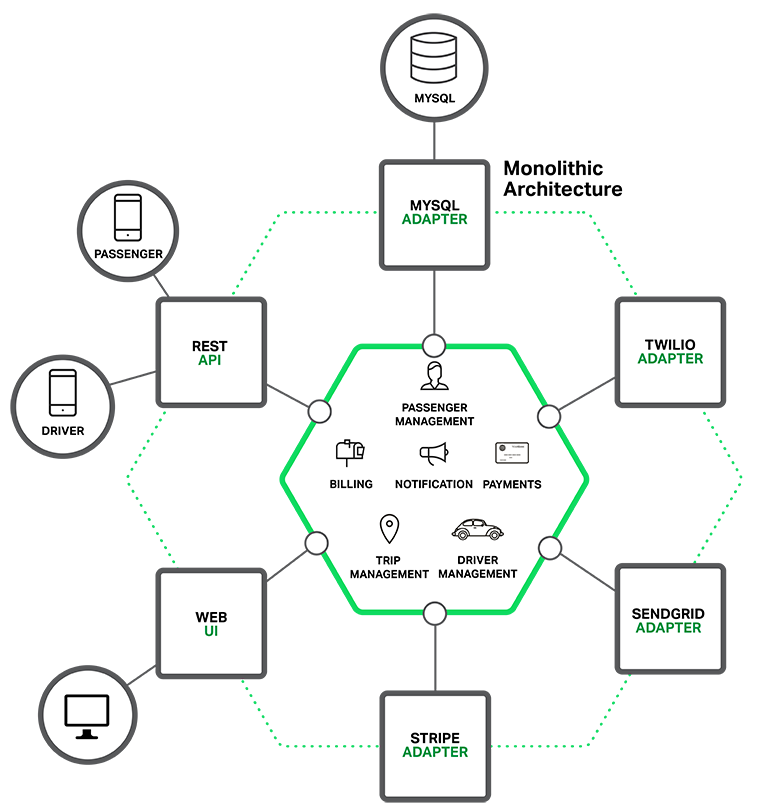
\includegraphics[width=\textwidth]{images/monolithic_application2.png}
	\caption{Monolithic application\footnotemark}
	\label{monolithic_application}
\end{figure}

\footnotetext{Source: \url{https://www.nginx.com/blog/introduction-to-microservices/}}

The server-side application handles all client requests, executes business logic, retrieves and update data from the database, and select and populate HTML views to be sent to the browser. This server-side application is a monolith (as shown in picture \ref{monolithic_application}) - a single logical executable. Any changes to the system involve building and deploying a new version of the application to the server. \cite{mf}

Monolithic application are typically developed by one, potentially big, team. All requests for change are aggregated into a single issue-tracking system from which the members of team pick their tasks. Likewise the whole team is sharing application's code-base through a single repository. When members pick their task, they pull current version of the code-base, compile it and start a local development instance on their machine. When they are done with their tasks, they merge their individual changes to the shared repository, thus conflicting changes may be common. In certain time current state of the code-base is marked with a version number and then compiled and deployed to the testing environment where it is tested and cultivated for some time before it is finally deployed to production.

Every change in large monolith can be cumbersome. Monoliths allow programmers to strongly couple their code. Change in one part of the application can immediately break something different or have unforseen consequences later. Refactoring of code becomes a pain.

Deployment of monolithic applications can be demanding due to conflicting  requirements on resources. Some of the modules can be processor-intensive, others memory-intensive, storage-intensive or network-intensive. Some modules may require ad-hoc software components like third-party software or different types of databases. Deployment environment then must supply all these needs at once which either leads to expensive or sub-optimal solution.

Monoliths also bring unnecessary overhead when scaling beyond a single machine, this is called horizontal scaling. There are two types of scaling: vertical and horizontal. Vertical scaling means that we are allocating more computing resources within a given machine to the application or you are upgrading the machine itself, this is the ordinary type of scaling. However, vertical scaling is always limited by technical limits of contemporary computer components. Furthermore price of those components rises exponentially together with their performance.

On the other hand with horizontal scaling we are running the same application on multiple machines at once. This solution also necessitate the use of intermediate machine called load-balancer which splits the incoming requests between all running applications on different machines. The downside of monolith is that even if the bottleneck of our application lies in a single component, we have to run multiple instances of the whole thing claiming more resources. Another problem is even if we utilize horizontal scaling, all the running monoliths share a single database, which then becomes bottleneck by itself.

Now when we look at the microservice architecture we will see a very contrasting mindset. Microservice architecture advocates slicing the monolithic application into well bounded, smaller application parts - microservices, that can each provide a part of the business value on their own. This process has been termed as \textit{"breaking the monolith"}. By providing business oriented APIs a collection of microservices then substitute the monolith.

As we see in picture \ref{microservice_application}, we broke the application from previous picture into individual components and exposed their APIs through API gateway to client-side applications. Each component can have numerous running copies on different computers (horizontal scaling) and API gateway serves as a load-balancer routing the incoming traffic to them. The only relation between different components is their communication using data exchange accomplished through the APIs they expose. How exactly you slice the business functionality depends on you, but you should try to make the microservices as independent as possible so they limit one another the least.

\begin{figure}[ht!]
	\label{microservice_application}
	\centering
	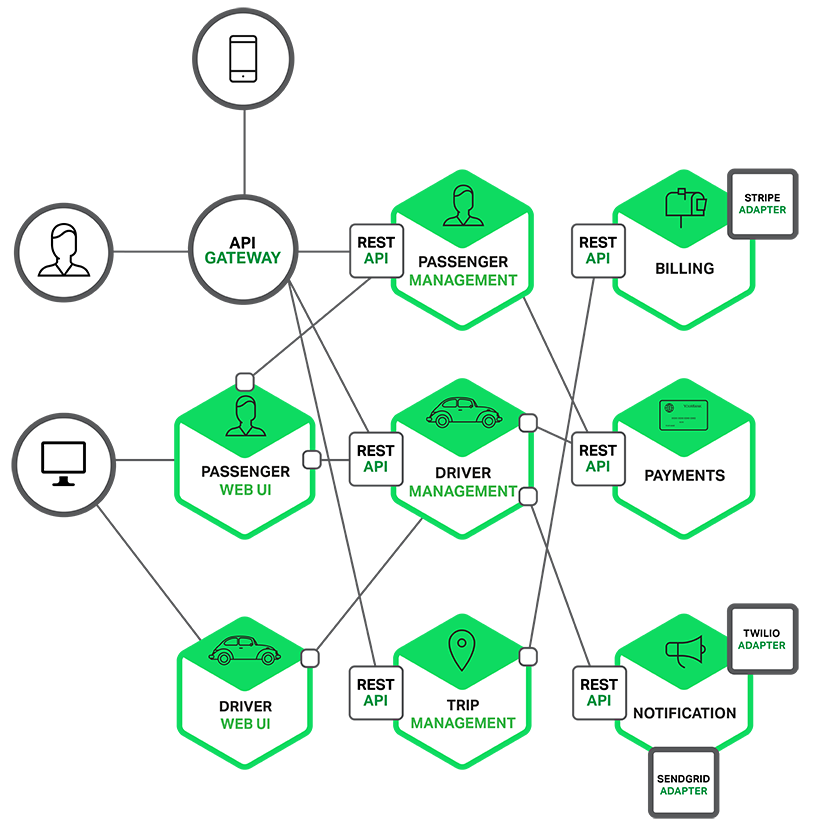
\includegraphics[width=\textwidth]{images/microservice_application2.png}
	\caption{Application as microservices\footnotemark}
\end{figure}

\footnotetext{Source: \url{https://www.nginx.com/blog/introduction-to-microservices/}}

Microservices architecture is not precisely defined in any book, it is not a standard. It is just a set of practices and recommendations that have been put together over time by companies and experts, who were facing common problems when building large scale applications. There are key principles that microservice application should stick to:

\subsection{Single responsibility principle}

One of the key principles is that a microservice should do only one thing and it should do it the best it can. This principle is inspired by the philosophy of UNIX where there are many small programs, each of them serves single small purpose and they work together to complete more complicated tasks.

This attitude contributes to microservices staying simple and seizable. They can be maintained by small teams, composed of only a handful of people, who have very good understanding of all aspects of the microservice. Code-base remains small, easy to change and to refactor.

\subsection{Isolation}

Microservices should be as isolated as possible. Isolation means that there are no common resource like a single database between microservices. It also means that every microservice has its own code-base. No relation exist between microservices other than a possibility of communication through arranged interfaces. Low coupling is crucial for many of the microservices benefits.

\subsection{Data ownership}

Part of the isolation principle is data ownership. Every microservice should be responsible for its own data and be able to manipulate it how it deems fit and even change it completely disregarding other microservices. Any other microservice can access these data only through the respective microservice that owns it.

Example of this may be e-shop application, where catalog microservice owns only data regarding all offered goods like their id, name, price, description and all kinds of attributes. Then we would have storage microservice that would own data quantity of each item in our stock. Cart microservice which would keep track of users shopping carts. Orders microservice which would take care of customer orders. Login service, images service, recommendations, invoices, etc.
Every microservice would store its data in its own database or hold it in a cache. This principle is necessary so that one shared database would not become another bottleneck of the application and single point of failure.

In picture \ref{decentralised_data} we can see difference in data handling between monolithic application and microservice application. On the left side all-inclusive application accesses one big database, performs some business functionality on it and returns the overall result to the user usually in the form of complete web page. On the right side individual microservices serve their respective data either to some front-end web server application or directly to client-side AJAX\footnote{Asynchronous Javascript and XML \url{https://en.wikipedia.org/wiki/Ajax_(programming)}} application or smartphone app. On the right, we can also see that there are two instances of the same microservice sharing one database.

\begin{figure}[ht!]
	\label{decentralised_data}
	\centering
	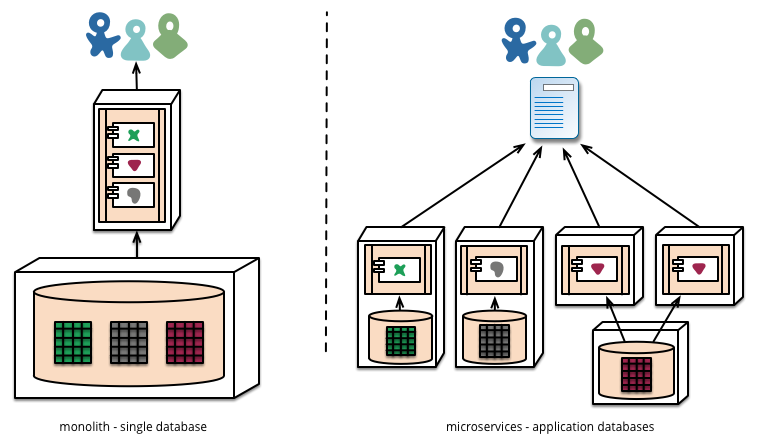
\includegraphics[width=\textwidth]{images/decentralised_data.png}
	\caption{Data division \cite{mf}}
\end{figure}

\subsection{Autonomy}

This principle says that the microservice should be able to exist on its own. Isolation is a prerequisite for autonomy. Only when services are isolated they can be fully autonomous and act independently. No other microservice in the system has to be running for a microservice to run.

Autonomous microservices open up flexibility around orchestration, scalability and availability. Each team and service can change its internal implementation details without impact across the rest of the system. Each service is developed, tested and deployed independently.

\subsection{Resilience}

With previous point ties another characteristic - resilience. Resilience is a capability to cope with unpredictable external changes or errors. A microservice cannot rely on other microservices or components that they will do their job.

In microservice world that encourages autonomy, there are many things that can go wrong. Instances of microservices start and stop on regular basis. It may even happen that in one moment there are no running instances of necessary microservice at all - for example when the whole system is just starting. Other microservice can return errors or unexpectedly stop short in the middle of a request. Since microservices are typically deployed across multiple machines in a network, all network problems need to be taken into account.

A microservices should also degrade gracefully. Which means that if another component it relies on wasn't able to provide its promised service, the reliant microservice gradually cuts some of its functionality but tries to leave the most of it, providing the best possible service it can in any given time.

\subsection{Light-weight communication}

Since microservices complete more complicated tasks only by cooperation, there are heavy demands on communication, both in frequency and volume. Thus communication between microservices must be as light-weight as possible. Communication protocols like SOAP that uses bloated XML format are undesirable. Instead microservices architecture recommends usage of protocols like REST that use shorter JSON format.

For example Netflix relies on even smaller message formats like Apache's Avro or Thrift and Google's Protobuf over TCP/IP for internal communication inside microservice systems. \cite{ma}

Some are taking things even further and advocate using an asynchronous message-oriented approach for communication between microservices. And instead of sending concrete serialized objects of agreed format, they send universal messages allowing for changes in content. This further helps to reduce coupling and allows refactoring.

\subsection{Continuous integration}

\begin{definition}[Continuous integration]
Continuous integration is a software development practice where members of team integrate their work multiple times per day and automatic build and test tools check the functionality of the application. \footnote{Continous integration by Martin Fowler \url{https://martinfowler.com/articles/continuousIntegration.html}}
\end{definition}

The goal of continuous integration is reduction of risk, it protects the development from surprises at the end of the development cycle. Waiting days or weeks to integrate code creates many merge conflicts, hard to fix bugs, diverging code strategies, and duplicated efforts. Continuous integration provides helpful feedback for both developers and customers.
\bigskip

\noindent\textbf{Key practices that enable continuous integration are:}

\begin{itemize}
\item \textbf{code-versioning} - use of modern code repositories like Subversion or Git is the standard in all good development practices
\item \textbf{frequent commits} - developers should commit their changes and checkout changes of others several times a day to reduce conflicts, it is even recommended not to use branching features for every task and work only on master branch
\item \textbf{automated builds and tests} - each integration (each commit to repository) should trigger an automated self-testing build that verifies the application using unit tests and other means to detect integration errors as soon as possible, it should be easy to see what changes made the build break
\item \textbf{fast builds} - the main point of CI is to provide rapid feedback, so keeping the build times as short as possible is imperative, luckily small scope and size of microservices favours this
\item \textbf{prepare to deliver} - after every successful build, or at least every day, new version of application should be pushed to testing environment so there is enough time before deploying to production when testers can spot out errors and stakeholders can adjust imperfections
\item \textbf{testing in clone of production} - having a test environment that is different from the production environment can lead to unexpected failures when finally deploying to production, so these two should be as much same as they can be, another solution is to have a pre-production environment
\end{itemize}

\subsection{Utilization of infrastructure}

Microservices architecture encourages pushing common concerns like management and monitoring of the running application to technical infrastructure and framework. Developers should only need to care about business logic.
Automated service discovery and routing should facilitate decoupling of services and enable easy upgrade and replacement.

\subsection{Conway's Law}

Conway's law is not a characteristic of microservice architecture but it is a difficulty that needs to be taken into account when designing one.

\begin{definition}[Conway's law]
Any organization that designs a system (defined broadly) will produce a design whose structure is a copy of the organization’s communication structure. \footnote{How Do Committees Invent \url{http://www.melconway.com/Home/Committees_Paper.html}}
\end{definition}

This finding warns against instinctive pitfall of designing individual microservices and the communication between them based on the preimage of existing teams in the company and their communication.

For example if we had three teams that are specialized respectively on UI, back-end and databases, they would be naturally inclined to develop three microservices - one for serving webpages only acting as a webserver, another executing all business logic and the last one for accessing the database. This would be a wrong distribution of responsibilities. Every change in the system would most certainly need modification of all three microservices.

\section{Microservices vs Service Oriented Architecture}

Microservice architecture is heavily inspired by service-oriented architecture (SOA). Some say microservices is a specialization of SOA. Service-oriented architecture is an interlink between monolithic systems and microservices. Both MSA and SOA are architecture patterns that place a heavy emphasis on services as the primary architecture component used to implement and perform functionality. However the crucial difference between them is that microservices architecture is a share-as-little-as-possible architecture pattern that places a heavy emphasis on the concept of a bounded context, whereas SOA is a share-as-much-as-possible architecture pattern that places heavy emphasis on abstraction and business functionality reuse. \cite{mvsoa}

SOA's focus on reuse means that one certain function should only exist in one place or that single service should handle it. Where things differ is definition of this function. This is where cohesion comes into play. Cohesion is the degree in which functionality in services belongs together. The highest cohesion is functional cohesion where the services contribute to a well-defined task or business capability. Microservices aim for high (functional) cohesion, whereas SOA uses low (logical) cohesion. Logical cohesion means that services are designed to provide similar tasks. This leads to services such as "data service"  which provides all communication with a database for the whole system. Now imagine the effects of this service going down. All parts of the system that persistently store data to database would stop working. With MSA the intention is to provide all aspects of business capability end-to-end, from data storage to user interface functions. So instead of having a "front-end service" and “data service” we have “customer service” and “shipping service” each with their own front-end and back-end part, including database.

MSA also strives for autonomy which not only means that a microservice should be able to run or function independently, but it also means that a microservice should be able to provide business value on its own.
\bigskip

\noindent\textbf{Lets summarize the key differences:}

\begin{itemize}
\item \textbf{Communication between services:} SOA usually has more dependent ESB (Enterprise Service Bus), whereas microservices use faster messaging mechanism, usually REST
\item \textbf{Programming style:} SOA encourages imperative programming, whereas microservices encourages responsive-actor programming
\item \textbf{Database:} SOA models tend to have an outsized relation database, while microservices frequently use NoSQL or micro-SQL databases (which can be connected to conventional databases)
\end{itemize}


\section{Advantages and disadvantages}

Now that we have a general idea of what microservices are, we should look at their benefits and pitfalls, and why is the industry so excited about them.

As Martin Fowler points out \cite{mf}, Netflix, eBay, Amazon, the UK Government Digital Service, realestate.com.au, Forward, Twitter, PayPal, Gilt, Bluemix, Soundcloud, The Guardian, and many other large-scale websites and applications have all evolved from monolithic to microservices architecture. So there must be certainly a good reason for these companies to prefer microservices architecture over monolithic architecture in some of their projects.\newpage

\subsection{Benefits of Microservices}
\bigskip

\noindent\textbf{Long-term maintainability}
\bigskip

Microservices attack the monoliths specific complexity in its tight coupling between individual, great amount of overall knowledge needed to make responsible changes to the system, technology lock-in, growing technology debt and so on.

When the monstrous monolithic application is broken up into manageable chunks it is easier for everyone in the project to work with the application and further maintain it. Maintainability is absolutely critical for success of big long-lasting projects and represents a great risk if not taken into account.
\bigskip

\noindent\textbf{Independent and horizontal scalability}
\bigskip

Evident advantage of microservice architecture is its adaptation to scaling. Isolation and autonomy of a microservice allow us to simultaneously run countless copies of it in addition to running them across different computers in a network.

So for example, if our application has to process computational-intensive task and this task is a responsibility of one of our microservices, we can run that given microservice as many times as we need to satisfy the demand for given task without scaling the whole application. And if one machine is not enough for the task, we can scatter the task on multiple computers.

Horizontal scaling is cheaper than vertical scaling and it renders the system more robust in case of hardware failure of one of the computers. Also readiness to scaling and fast start-up of small microservices allows our application to accommodate sudden spikes of service demand by starting additional instances of given microservice and vice-versa, when the demand falls of, the application can automatically stop superfluous instances to save resources.
\bigskip

\noindent\textbf{Continuous delivery}
\bigskip

Acceleration of changes in our everyday world go hand in hand with increasing demands on companies that are facing frequent changes in their areas of business. Nowadays the ability to readily react to these frequent changes is becoming critical competitive advantage. As we can see in picture \ref{fast_fish} taken from Reactive Microservices Architecture \cite{rma}, big mature companies that so far dominated their respective business sector can quickly become prey to their faster, more agile competitors.

\begin{figure}[ht!]
	\label{fast_fish}
	\centering
	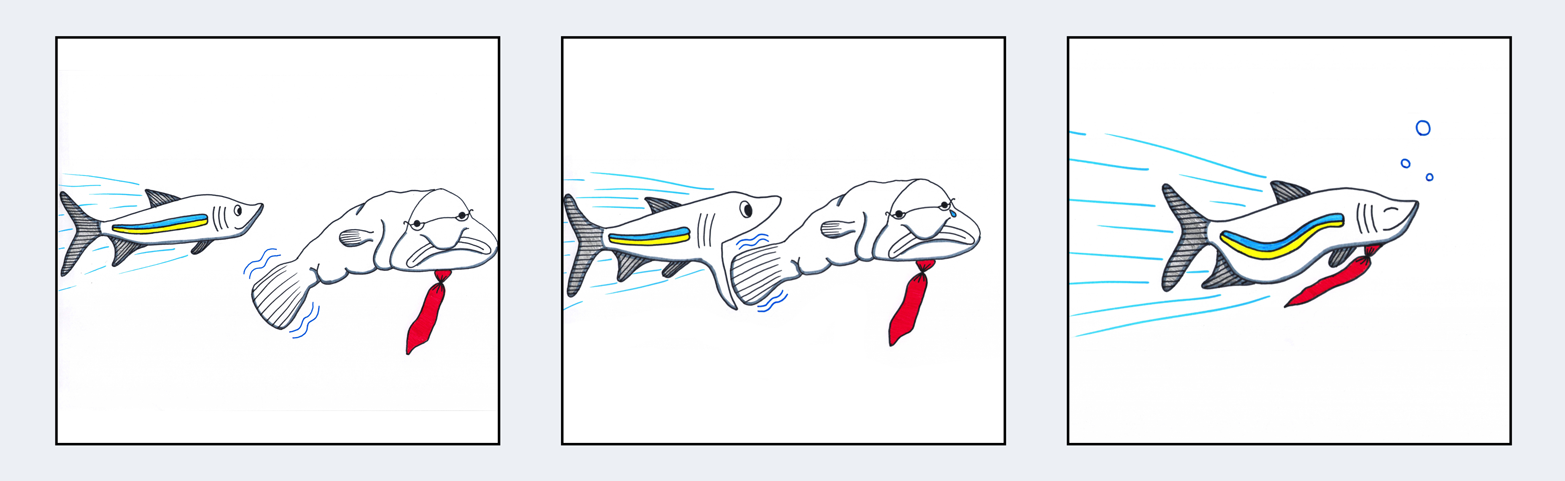
\includegraphics[width=\textwidth]{images/fast_fish.png}
	\caption{Slow fish versus fast fish \cite{rma}}
\end{figure}

One of the key benefits, for which more and more companies are adopting microservices, is the short time span between a request for change and its deployment that they offer. This is thanks to proficiency in continuous delivery.

\begin{definition}[Continuous delivery]
Continuous Delivery is a software development discipline where you build software in such a way that the software can be released to production at any time. \footnote{Continuous Delivery by Martin Fowler \url{https://martinfowler.com/bliki/ContinuousDelivery.html}}
\end{definition}

So continuous delivery enabled by continuous integration is the ability to quickly roll-out software updates to production. The biggest risk to any software effort is that you end up building something that isn't useful. Continuous delivery helps to avoid this by enabling early user feedback. Also since it's recommended to continuously roll-out small updates to the production, there is less to go wrong and it's easier to fix should a problem appear.

The isolation and autonomy principles empower fast and flexible microservice deployment and upgrade. They make it possible for new versions of microservices to be taken into production independently of changes to others, allowing us to safely roll-out or revert changes incrementally - service by service. What's more we can roll the changes out instance by instance of the same microservice and slowly redirect the traffic to the new version, which effectively means zero downtime. That is a big deal for systems that have very strict availability requirements.

With the flexibility of routing and deployment it is also easy to exercise canary release. Canary release is a technique for reduction of risk, in which you expose new versions only to a fraction of the users at first. You can choose a random sample of users or you can target certain groups of people according to region, age, sex, etc. and get their feedback. And only if those users are happy with the new version, you make the update available to all users.
\bigskip

\noindent\textbf{Technology diversity}
\bigskip

Since the only relation between individual microservices should be a network communication through an agreed interface that should be language-agnostic, developers can take advantage of technology diversity. This benefit also eliminates long-term commitment to a single technology stack.

It is possible for every microservice to be written in different programming language, use different framework or even be developed for different platform like x64 or ARM. ARM architecture is usually less power consuming, which can be useful in IoT\footnote{Internet of Things - \url{https://en.wikipedia.org/wiki/Internet_of_things}} applications. Each microservice can leverage the use use of database type that is the most suitable for its data, be it relational or non-relational database.\newpage

\subsection{Drawbacks of Microservices}
\bigskip

\noindent\textbf{Architecture complexity}
\bigskip

While microservices take away the complexity of big monoliths they bring another type of complexity that is inherent in the microservice architecture itself. It arises from the fact microservices are distributed system, so there are many things that need to be taken care of.

The deployment environment is much more complicated. Now there is no application server, to which we simply deploy our WAR file. We need a mature operations team and employ new middleware and tools to manage numerous microservice instances, which are being redeployed regularly.
\bigskip

\noindent\textbf{Network communication}
\bigskip

Microservices heavily depend on network communication which always brings many problems to the table. There is no simple invocation of method in different module via language specific call, we have to use remote calls to communicate with another microservice.

If all things work perfectly, the network call may take a multitudes of time. Even inter-process network calls between instances on the same machine take substantial amount of time compared to method calls inside a single process. So developers need to find a compromise between excessive division of business functionality into individual microservices and its aggregation.

What's more in network space we never know what can go wrong on the other side or if our message ever reach its destination, so we need to take care of every possibility. This alone brings a massive amount of complexity to microservice architecture. We need to have strong resilient mechanisms in every microservice, implement timeouts and fallbacks, and check incoming data.
\bigskip

\noindent\textbf{Data consistency}
\bigskip

Since microservice architecture promotes ownership of data associated to each microservice and not having a single database for everything, data consistency becomes a challenge.

Business transactions that update multiple business entities are fairly common. In microservice architecture these business entities can belong to different microservices. Using distributed transactions should be put to use only for critical data because of the CAP theorem\footnote{\url{https://en.wikipedia.org/wiki/CAP_theorem}}. All other data should do with eventual consistency\footnote{\url{https://en.wikipedia.org/wiki/Eventual_consistency}}.
\bigskip

\noindent\textbf{Testing complexity}
\bigskip

If we omit unit testing that verifies the workings of internal components and should have the same complexity as in monoliths, then microservice architecture has more complicated overall testing.

In monolithic application with modern frameworks its trivial to write tests that start the application and test its external APIs. However, with microservices we need to also test inter-service communication and application as a whole. To do that we have to launch the tested microservice and any other microservices it depends on, or their stub. We may also need to test compatibility of various versions of microservices.
\bigskip

\noindent\textbf{Summary\newline\newline}

Microservice architecture is ideal for big, demanding, robust systems. The common problems that companies were facing were related to size of the system. Microservice architecture is designed to solve problems of systems which grew in size beyond the boundaries that were initially defined when the system was designed. Microservices are also ideal for applications with very high load and availability demands.

There are no silver bullets, like every other technology, microservice architecture has its advantages and disadvantages and so it's advisable in some situations and inappropriate in others. In picture \ref{productivity} we can see fitness of microservices with regard to applications complexity.

\begin{figure}[ht!]
	\label{productivity}
	\centering
	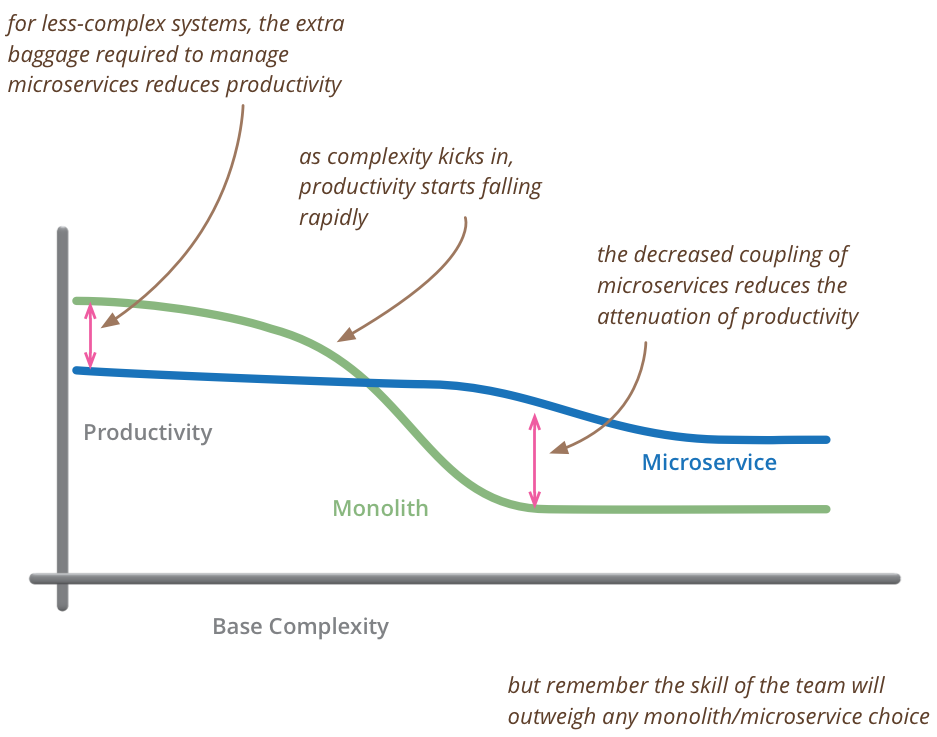
\includegraphics[width=\textwidth]{images/complexity_productivity.png}
	\caption{Relationship between complexity and productivity\footnotemark}
\end{figure}

\footnotetext{Source: \url{https://martinfowler.com/microservices/}}

\section{Containers}

In traditional approach we built one binary of our application and deployed it to the server which needed to be correctly configured (correct permissions, environment variables, etc.) and include everything that our application need for functioning. Likewise we needed to be careful so that various changes don't impact other applications also running on the same server. With microservices this becomes much more complicated.

After we break our application we end up with many moving pieces. Services, binaries, different configurations etc. We need a technique to elegantly wrap our application to integrated packages that are easy to deploy and simultaneously segregate our application from the rest.

In the past virtual machines\footnote{\url{https://en.wikipedia.org/wiki/Virtual_machine}} were used for this need. Virtual machines have their foundation in some computer areas, but they are cumbersome for our purpose. Each virtual machine virtualizes an entire hardware and takes up a lot of RAM and CPU. Images of virtual machines are huge because they not only contain the application, but the whole operating system with the required drivers and other redundant parts. Virtual machines are hard to manage, patch, and change. Building a new image as well as starting it takes a long time, which is not ideal in microservice fast changing applications.

The reason microservice architecture is financially and operationally feasible has lot to do with containers. Containers bear much less overhead and enable you to deploy a lot more applications onto a single physical server than virtual machines do. They are also much more agile, build fast and start in milliseconds. Unlike virtual machines, containers virtualize the operating system kernel, not the hardware. So the applications in containers must all work on given kernel and there is somewhat bigger security risk if one container is compromised with superuser privileges.

Docker\footnote{\url{https://www.docker.com/}} is an open-source project which brought the container principle to a mature level by providing additional layer of abstraction and tools. Docker made containers easier and safer to deploy and use than previous approaches. In picture \ref{vm_vs_docker} we can see the difference in virtualization between Docker and virtual machines.

\begin{figure}[ht!]
	\label{vm_vs_docker}
	\centering
	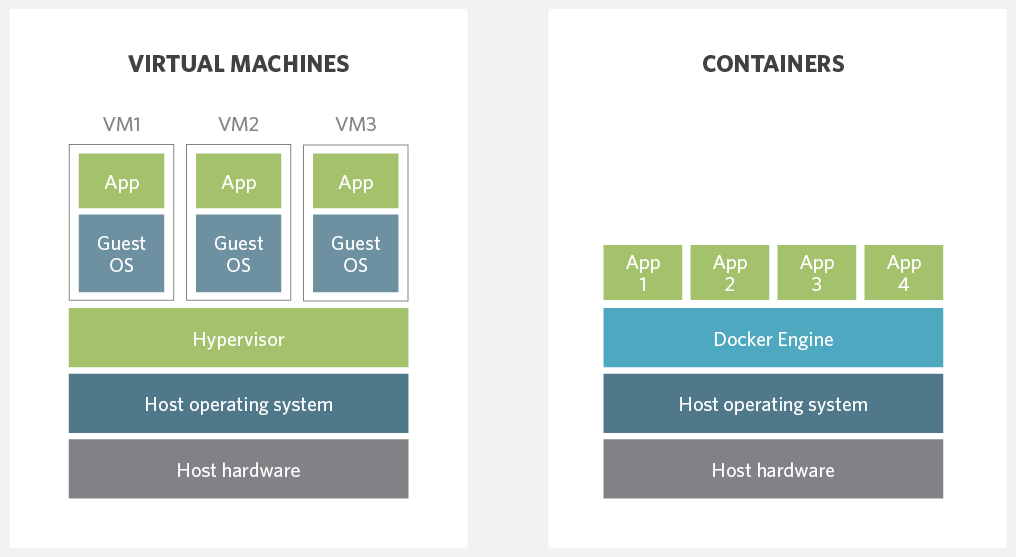
\includegraphics[width=\textwidth]{images/virtual_machines_vs_containers.png}
	\caption{Difference between virtual machines and containers\footnotemark}
\end{figure}

\footnotetext{Source: \url{http://searchservervirtualization.techtarget.com/answer/Containers-vs-VMs-Whats-the-difference}}

However Docker alone only enables us to deploy and manage containers within the scope of a single machine. Big applications need to scale and operate across multiple machines and that's where container schedulers come in. Container schedulers automate deployment, scaling and management of containerized applications in our cluster of computers. They take care of deciding when and on what machine to start and stop our containers depending on the given application configuration. There are three known container schedulers: Docker's Swarm, Apache's Mesos and Google's Kubernetes\footnote{\url{https://kubernetes.io/}}, which is the most widely used one. Kubernetes project is also extended by OpenShift\footnote{\url{https://www.openshift.com/container-platform/}} project that further dulcifies management with web interface and other tools.

\section{SilverWare}

SilverWare\footnote{\url{https://github.com/SilverThings/SilverWare}} is one of the frameworks that make it easy for developers to start creating microservice applications by providing fundamental parts needed for operation of most microservices. SilverWare is written in Java and exercises minimalistic easy-to-use approach. It only integrates few powerful libraries and leaves it on the developer which ones to use. Thanks to that, the compiled application is very small and take a lot less memory when running than other most known platforms, like Spring Boot or WildFly Swarm. SilverWare is made up of modules called providers. Every provider adds a part of a functionality to the application that we are building.

\subsection{CDI Microservice Provider}
The crucial and most used provider is the CDI Microservice Provider. This provider is also dependency to many other providers. It uses CDI\cite{cdi_tutorial} reference implementation Weld\footnote{\url{http://weld.cdi-spec.org/}} to equip developers with dependency injection mechanism for easy interconnecting of their microservices. Every class that represents a single microservice has to be marked with @Microservice annotation. In this microservice class we can then seamlessly call functions of other microservices by injecting them to class fields marked with @MicroserviceReference annotation. CDI provider accomplishes this by implementing its own CDI Weld extension that scans for injection points in managed microservice beans.

\subsection{Cluster Microservice Provider}
By default CDI provider injects only instances of microservice classes running in the same SilverWare instance (same JVM) which isn't too much useful. Therefore extension of the purpose of the CDI provider is the Cluster Microservice Provider. It uses JGroups\footnote{\url{http://jgroups.org/}} project for interconnecting individual SilverWare instances in configured cluster and therefore enabling developers to inject remote microservices.

\subsection{HTTP Server Microservice Provider}
Another important module is the HTTP Server Microservice Provider which allows deploying a servlet into a servlet container and providing REST interface. It uses fast and lightweight Undertow\footnote{\url{http://undertow.io/}} as an underlying web server. With this provider we are able to easily expose REST interface in any microservice by using standard @Path, @GET, @POST, @Produces annotations.

\subsection{REST Client Microservice Provider}
Then we have the REST Client Microservice Provider, which simplifies use of foreign REST APIs. Developers can define interface that represents given API with its paths, arguments and results and then use this interface as a type of class field annotated by @ServiceConfiguration with URL to the API. Afterwards the developer is able to use the API simply by calling functions of the interface.

\subsection{Hystrix Microservice Provider}
Next we have Hystrix Microservice Provider, which allows developers to easily add fault tolerance mechanisms to their projects. As the name tells, it uses Hystrix \footnote{\url{https://github.com/Netflix/Hystrix}} latency and fault tolerance library and provides simple annotation-based configuration. @Cached for caching responses, @CircuitBreaker for stopping pointless request to inaccessible or failing components, and other useful annotations.

\subsection{Other microservice providers}
Other providers include Vertx Microservice Provider enabling developers to take advantage of Vert.x{\url{http://vertx.io/}} event driven and non blocking framework, Camel Microservice Provider for easy connecting of microservices to Camel{\url{http://camel.apache.org/}} routes, ActiveMQ Microservice Provider for integrating with Java Message Services, Drools Microservice Provider for integrating with business rules management system Drools, Monitoring Microservice Provider for reporting execution times and count of functions invoked through CDI to JMX and Jolokia Microservice Provider for making JMX available through REST interface.

\subsection{Build}
SilverWare compiles our application to a single all-including JAR file, which is easy to run anywhere Java is installed and is well suited for deployment in containers. This is a widely used manner of building microservices in all Java microservice frameworks.

\chapter{Monitoring of microservices}

Monitoring of our application is necessary for many reasons. First we need to know if the application is even running, we need to know if there are any problems that have to be solved and where they are specifically. Then we need to know the current load of the application, how is it performing, what are its bottlenecks. Then we would like to know how are the users working with our application, we may be interested in various statistics about the usage of individual components and such. Also monitoring is needed for our application if it has to fulfil a service-level agreement.

Monitoring of monoliths is unsophisticated. Usually we only have one powerful machine hosting an application server running our application. So we only need to care about one hardware, which we fully control, its performance and configuration and we have simple access to numerous runtime information of our application provided by the application server administration interface. Also every custom monitoring is accessible on this machine in one place.

While microservices distributed architecture delivers significant benefits, it is much more complex system with many moving parts. Inner workings of the system are not so clear and accessible as with monoliths. By default there is no single administration point providing an easy survey of various statistics of the application. In large applications there may be thousands or even more microservices running at the same time on different machines across different networks. What's more, these microservices can swiftly come up and die down in a matter of seconds. Gathering overall information about the system in such environment becomes difficult. So we are in need of some central point where we could view aggregated monitoring information from individual microservices transformed into some useful results.

\section{Monitoring patterns}

To have a better idea of monitoring and what it includes, there is a great website\cite{ms_patterns} which breaks down design patterns used in microservices into a well arranged graph. In picture \ref{observability} we can see six main areas of observability (monitoring). All solutions for these patterns should have as little runtime overhead as possible.

\begin{figure}[ht!]
	\label{observability}
	\centering
	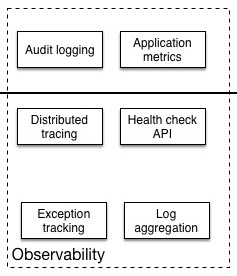
\includegraphics{images/observability.jpg}
	\caption{Design patterns in microservice monitoring\cite{ms_patterns}}
\end{figure}

\subsection{Audit logging}
Audit logging Concerns the behavior of our users. Its useful, sometimes necessary, to have a record of user actions for security, customer support or other reasons. Audit logging is manged manually in business code by developers.

\subsection{Application metrics}
We are most certainly interested in how are our individual components performing. We may want to know the usage of some components, statistics about successful and failed requests, amount of time it take for some actions to complete and other custom statistics, for this purpose serve metrics. Most of the metrics are usually managed manually by developers in business code. Some basic metrics like usage of processor, memory and disk can be provided by either container schedulers or separate utilities inside containers like collectd\footnote{\url{https://collectd.org/}}.

We then aggregate these metrics and create useful reports from them, fire alerts if something goes wrong and draw various monitoring graphs for operations team. Metrics are also used for evaluation of service-level agreements.

It has to be taken in mind that we cannot monitor everything, in big systems with many microservice instances this could result in ten-thousands of metrics per second and cause overload of both our system and our perception. We need to focus only on metrics that represent business value or key performance statistics, which can help in further development.

\subsection{Distributed tracing}
Tracing helps us understand the behavior of our application. Requests to our application often span many different microservices and in each of them perform one or more operations, database queries and such. External monitoring of responses or metrics for individual microservices will not tell us the reasons why similar request are sometimes fast and sometimes too slow. We need to follow the requests through the whole system and log elapsed time of individual operations and other useful intermediate info.

This is done by assigning unique ID to every external request and passing it together with every subsequent call inside our application. Individual microservices are then able to record relating information for each request and send them together with the request ID to some centralized tool. This tool then aggregates all the data and displays them in some well arranged manner or even shows dependency graph between our microservices. 

Tracing can be generally managed by the infrastructure or framework regarding calls between microservices, but many times a cooperation of developer is needed to add useful relevant information to the traces.

\subsection{Health check API}
We cannot presume that our microservice is running just because the container it's in is running. And we cannot even presume that the microservice is working and is able to fulfill its duty just because it is running. 

For this reason we need health checks in our microservices. Health checks are repeating audits of microservice capability to serve incoming requests. They usually repeat in matter of seconds and expose the results of audit to a REST API of the microservice for easy access, typically something like \textit{http://156.184.120.95/health}

Examples of some health checks could be:
\begin{itemize}
\item \textbf{locked threads} - are there any deadlocks\footnote{\url{https://en.wikipedia.org/wiki/Deadlock}} in our microservice (JVM provides easy access to this information)
\item \textbf{database} - is the database available, do we have free database connections
\item \textbf{connection} - is our microservice connected to other microservices, are they responding
\item \textbf{host} - is there enough disk space on the host, isn't the host running out of memory
\item \textbf{application logic} - are we able to run all business operations, are there any missing resources
\end{itemize}

Results of health checks can be gathered by some monitoring tool, however they primarily serve as an indication of operation for container schedulers. Container scheduler can see a container running, but it has no idea if the microservice instance in it initialized alright or if it's working as supposed to. For that reason we can define a health check API to container scheduler and if the API is inaccessible or returning some errors, the container scheduler knows it cannot route incoming request to the container and will try to restart it.

\subsection{Exception tracking}
In microservice architecture things are destined to fail, at least temporarily. Connection times out, data aren't synchronized, some service isn't momentarily available. Microservices can generate a lot of exception. So we can use a tool that aggregates these exception, de-duplicates, filters the expected ones and displays the problematic ones for further investigation by developers. This pattern does not need any assistance from developers in business code.

\subsection{Log aggregation}
This is self-explanatory. Our microservices probably generate some log files, which contains errors, warnings, info and debug messages. We need a tool to gather these log file in one place with filter and search capabilities. The tool should also have a alert settings if we need to be notified of some events.

\section{Monitoring solutions}

I focused mainly on open-source monitoring solutions that I could integrate into SilverWare. However, there also exist many proprietary solutions, which arguably do a better job as more versatile tools. These solutions put themselves into Application Performance Monitoring (APM) category representing universal all-including tools for monitoring, which on top of basic metrics and tracing capabilities sometimes offer more advanced features like artificial intelligence, to spot out interesting data in lots of metrics and help with finding the root cause of problems. Some of these proprietary solutions are Instana, Netsil, AppDynamics, DynaTrace, they offer integration with many container schedulers, programming languages, frameworks, databases, webservers, alerting and other tools.

\subsection{OpenTracing}

Tracing is probably the most useful pattern in microservice architecture. Many problems cannot be solved by other metrics because they do not follow the whole story of what has happened in our application step by step. There are already many distributed tracing solutions available. Most solutions create part of the traces automatically by recording invoked functions, however developers usually need to add their own intermediate steps to the trace and other relevant info. So they end up linking their code with the chosen tracing solutions putting the application under vendor lock-in, which is always good to avoid in the long run.

OpenTracing\footnote{\url{http://opentracing.io/}} is a vendor neutral open standard for distributed tracing. It is a very young project. It abstracts the tracing API from actual underlying vendor implementation, meaning that we call universal best-practice functions defined by OpenTracing standard and the underlying implementation tries to make the best use of them. At anytime we can easily change the implementation. OpenTracing does not guarantee us that we can use different tracing implementations in different components, but this is not usually needed, because we typically want to have all tracing data available in single tool.

So far OpenTracing has defined tracing API in Go, JavaScript, Java, Python, Objective-C, C++. It has integrations in Spring Boot, Dropwizard, Django, Go Kit, Grpc and others in various state of development and has tracing implementations for Zipkin, Hawkular APM, Appdash, Instana, Jaeger, LightStep.

OpenTracing has a very simple scheme. Its basic element is a \textit{Span} object. \textit{Spans} represent individual traced operations. \textit{Spans} always have name and time of start and end. They can hold additional information in form of key/value pairs called \textit{tags}, some of which are widely understood by tracing implementations and apply to the the whole span \textit{Spans} can also hold key/value logs, which apply to specific time.

\textit{Spans} can start other \textit{spans} in serial or parallel way, which is achieved by defining a newly created \textit{span} as a child of parent \textit{span}. That way the child \textit{span} inherits its parent's transaction id. Interconnected \textit{spans} create a acyclic graph that composes a \textit{trace}. \textit{Traces} tell the complete story of a transaction as it propagates through our system.

Recorded traces are typically displayed in the tracing tool in form of line graph showing all trace's internal spans in context of time and their serial or parallel nature as in picture \ref{opentracing2}.

\begin{figure}[ht!]
	\label{opentracing2}
	\centering
	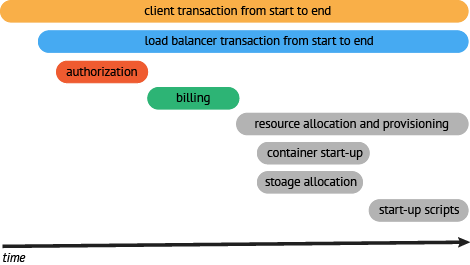
\includegraphics[width=\textwidth]{images/opentracing2.png}
	\caption{Trace with 8 spans \cite{opentracing}}
\end{figure}

Central element in the OpenTracing API is the \textit{Tracer} interface that needs to be implemented by tracing provider chosen by developer. Tracer interface has 3 functions:

\begin{itemize}
\item \textbf{buildSpan(String operationName)} - returning \textit{SpanBuilder} for creation of new \textit{Span} with given name and possibly as a child of another \textit{Span} or \textit{SpanContext}
\item \textbf{inject(SpanContext spanContext, Format<C> format, C carrier)} - for injecting a \textit{Span}'s \textit{SpanContext} into a `carrier` of a given type, presumably for propagation across process boundaries
\item \textbf{extract(Format<C> format, C carrier)} - for extracting that \textit{SpanContext} from a `carrier` after a propagation across a process boundary
\end{itemize}

By propagation across process boundaries we particularly mean calls between microservices through various means like REST request, message sending, RPC, etc. What the OpenTracing implementations choose to store in these Carriers is not formally defined by the OpenTracing specification, but the presumption is that they will encode some "tracer state" about the propagated \textit{SpanContext} like \textit{span\_id} and \textit{trace\_id} to later put the spans together into a trace when they are reported from different components. \textit{SpanContext} After the \textit{Span} is build using the \textit{start()} function of \textit{SpanBuilder} we can manipulate it using these methods (not complete list):

\begin{itemize}
\item \textbf{SpanContext context()} - returning Span's \textit{SpanContext}
\item \textbf{setTag(String key, String value)} - for setting tracing tags
\item \textbf{log(long timestampMicroseconds, Map<String, ?> fields)} - for setting span logs
\item \textbf{setBaggageItem(String key, String value)} for binding custom developer string values to the span, which will get transfer in \textit{SpanContext} across process boundaries together with 
\end{itemize}
\newpage

Logs are mostly used to store tracer implementation specific events, human readable messages and details of possible errors. Regarding universal tags, some of the widely understood are\cite{opentracing_spec}:

\begin{flushleft}
\renewcommand{\arraystretch}{1.65}
\begin{tabular}{| l | c | p{8cm} |}
\hline
\textbf{Tag name} & \textbf{Type} & \textbf{Usage} \\ \hline
component & string & Name of the component that created the span \\ \hline
error & bool & True if there was an error in operation represented by the span \\ \hline
http.method & string & HTTP method of the request, for example "GET" or "POST" \\ \hline
http.url & string & URL of the request resource, for example "http://domain.net/path/to?arg=val" \\ \hline
peer.hostname & string & \mbox{Remote hostname, for example} \mbox{"internal.dns.name"} \\ \hline
peer.port & integer & Remote port \\ \hline
span.kind & string & Either "client" or "server" for the appropriate roles in an RPC, and "producer" or \mbox{"consumer"} for the appropriate roles in a messaging scenario \\ \hline
\end{tabular}
\end{flushleft}

\subsection{Zipkin}

Zipkin\footnote{\url{http://zipkin.io/}} is an open-source distributed tracing tool supporting OpenTracing. It gathers traces sent to it and manages both the collection and lookup of this data. User is able to filter or sort all traces based on the application, length of trace, annotation, or timestamp. Zipkin can presents concrete traces in the form of previously described graph and after clicking on spans, it displays additional information like their tags. Zipkin can also produce a very simple dependency graph between components based on the recorded traces. You can choose to save the data either in MySQL, Cassandra or ElasticSearch database.

\subsection{Hawkular APM}

Hawkular APM\footnote{\url{http://www.hawkular.org/hawkular-apm/}} is an open-source metrics and tracing tool with support for OpenTracing. It does not present the traces in forementioned span "lines graph", however it can display more communicative dependency graph between components for whole application and for individual traces. It can also produce many different graphs from traced and metered business transactions.

\subsection{Metrics library}

Metrics\footnote{\url{http://metrics.dropwizard.io}} is an open-source library for measurements, which is a part of the Dropwizard framework. It is probably the best metrics library for Java. It is very easy to use, has modules for common libraries like Jetty, Jersey, Apache HttpClient and can report metrics to JMX, Graphite or Ganglia and many other. It provides various metric types and also a health check API.

Central part of the library is \textit{MetricRegistry} class. We register all our metrics to created instance of this class and it reports their values in given intervals to chosen reporters. The list of supported metrics follows\cite{metrics}:

\begin{itemize}
\item \textbf{Gauge} - the simplest type, when reported it returns just a current integer value from given function
\item \textbf{Counter} - a simple integer metric, provides \textit{inc(value)} and \textit{dec(value)} methods for incrementing and decrementing its value
\item \textbf{Histogram} - a histogram measures the distribution of values in a stream of data, it provides values like min, mean, max, standard deviation, and  75\%, 95\%, 99\% quantiles. It provides a \textit{update(value)} for adding a new value to its reservoir of cached values from which it computes results. Reservoirs can have miscellaneous implementations, some cache results for specified shorter time, some specified amount of ticks, others use more advanced algorithms to provide more long-term representative results.
\item \textbf{Meter} - a meter measures the rate at which an event occur, it provides mean rate and exponentially-weighted moving average rates of 1, 5 and 15 minutes. It has a \textit{mark(value)} function to add a number of new occurences
\item \textbf{Timer} - a timer is basically a histogram of the duration of a type of event and a meter of the rate of its occurrence, it has a \textit{time()} function, which is called at the start of the measured segment and returns a \textit{Timer.Context} object on which we need to call a \textit{stop()} method at the end of the measured segment
\end{itemize}

A sample output of the console reporter can look like:
\begin{lstlisting}[caption = Metrics console reporter output, label = spanmanager, style=eclipse_java]
-- Histograms --
name1
count = 1540
min = 11.95
max = 102.61
mean = 26.21
stddev = 40.54
median = 35.00
75% <= 20.00
95% <= 18.32
98% <= 16.84
99% <= 13.40
99.9% <= 12.05
 
-- Meters --
name2
count = 2012
mean rate = 175.87 events/second
1-minute rate = 0.00 events/second
5-minute rate = 25.34 events/second
15-minute rate = 56.86 events/second
\end{lstlisting}
\newpage
A request to health check API can return something like:\newline

\begin{verbatim}
{"deadlocks":{"healthy":true},"database":{"healthy":true}}
\end{verbatim}

\subsection{Graphite}

Graphite\footnote{\url{https://graphiteapp.org/}} is an open-source metrics monitoring tool. Graphite has a vast amount of collection agents and integrations to other visualization and monitoring tools. Graphite consist's of three parts:

\begin{itemize}
\item \textbf{Carbon} - a high-performance service that listens for time-series data either in plaintext format, pickle format or as AMQP messages
\item \textbf{Whisper} - a simple database for storing time-series data in multiple defined precisions over defined time
\item \textbf{Graphite-Web} - a web interface and API for rendering graphs and dashboards
\end{itemize}

Graphite is push based tool, meaning components must send their metrics to it. Metrics are reported to Graphite under their unique name delimited by a dot together with value and time. Reporting a current value of some metric can be as easy as:\newline

\begin{verbatim}
$ echo "metric.name 123 `date +%s`" | nc localhost 2003
\end{verbatim}

\subsection{Prometheus}

Prometheus\footnote{\url{https://prometheus.io/}} is another open-source metrics monitoring tool. Unlike Graphite it has a pull based approach. Microservices have to provide interface, which Prometheus scrapes for values. Prometheus scans a range of IP addresses, set in configuration, on which it hopes to find running microservices.

Prometheus is time-series database just like Graphite, but in addition to simple name-value-time single record it allows the data to be extended by tags. Some tags are implicit like the hostname from which the record has been scraped and some can be added by developer. Users can then filter the values according to these tags.

\subsection{Grafana}

Grafana\footnote{\url{https://grafana.com/}} is an open-source dashboard for unifying monitoring data. It has very fancy UI and has great amount of data-source integrations from which it can harvest data. It also offers many plugins and alerting capabilities.

\chapter{Monitoring extension for SilverWare}

Since there are some good monitoring tools and libraries already available, I chose to follow the most repeated and useful advice in software development, which is "Don't reinvent the wheel." Already implemented and widely used solutions are usually well documented and tested by their numerous users. These popular solutions also spring communities of users, which help each other solving various problems on forums and further contribute to maturing of the solution.

I decided to extend the SilverWare platform with two microservice providers which in my opinion are the most essential in microservice monitoring, using the open-source libraries described in previous chapter. First provider called OpenTracing Microservice Provider, which enables SilverWare developers to easily trace their application. And the second called Metrics Microservice Provider, which enables developers to create microservice health checks and custom metrics for reporting to Graphite or other tools.


\section{OpenTracing Microservice Provider}

For tracing provider I aimed to provide very easy access to tracing through static \textit{Tracing} utility class and extend the basic core API of OpenTracing with some useful contribution projects managed by OpenTracing community.

First I decided to include the \textit{GlobalTracer} project, which already became part of the core library while I was writing this thesis. \textit{GlobalTracer} is a static wrapper class which simplifies the plugging of \textit{Tracer} implementation and provides easy access to it throughout the whole application. It has a static method \textit{register(tracer)}, that registers a developer managed \textit{Tracer} implementation and a static method \textit{get()}, that returns singleton instance of the \textit{GlobalTracer}. \textit{GlobalTracer}'s functions \textit{buildSpan(name)}, \textit{inject(spanContext)} and \textit{extract(spanContext)} then propagate to wrapped tracer implementation.

Next I decided to include the \textit{SpanManager} project, that simplifies handling of \textit{Spans} throughout the code. To add tags, logs and create child spans you always need access to the current \textit{Span} instance, that encompasses your operation. Normally you would need to pass that instance to every function call and every function would have to accept it as an argument. However, \textit{SpanManager} enables us to remember and access given \textit{Span} across all functions during the execution of the same thread.
It does this by utilizing Java's \textit{ThreadLocal}\footnote{\url{https://docs.oracle.com/javase/7/docs/api/java/lang/ThreadLocal.html}} class, which holds a map of values binded to \textit{Thread} objects.

\textit{SpanManager} provides 3 functions. \textit{activate(span)} sets given span as current thread managed span and returns a \textit{ManagedSpan} instance containing a \textit{deactivate()} function to later unmanage the \textit{Span}. \textit{current()} returns the current thread \textit{ManagedSpan} with a \textit{Span} instance in it, or an empty \textit{ManagedSpan} if there is currently no activated \textit{Span}. You are able to stack active spans by calling \textit{activate(span)} on different \textit{Spans}, always the last still active \textit{Span} in the stack is returned by \textit{current()}. \textit{clear()} function deactivates all managed spans of current thread. In following example we can see creating a new \textit{Span} for request and its child \textit{Span} with the help of \textit{SpanManager} and \textit{Tracing}.
\newline

\begin{lstlisting}[caption = Usage of SpanManager, label = spanmanager, style=eclipse_java]
public class SpanManagerExample {
	public String handleRequest(Object object){
		Span span = Tracing.createSpan("name1");
		Tracing.spanManager().activate(span);
		...
		String result = innerFunction(object);
		...
		span.finish();
		return result;
	}
	public String innerFunction(Object object) {
		Span parentSpan = Tracing.spanManager().current();
		Span childSpan = Tracing.createSpan("name2", parentSpan);
		...
		childSpan.finish();
		return result;
	}
}
\end{lstlisting}

Another project I incorporated is JAX-RS integration for automatic creation of server spans on provided REST resources and client spans on REST client requests. I've taken in mind SilverWare's low coupling principle that distinguishes it from other framework and designed the solution so it doesn't add any dependency between provider modules.

I extended \textit{HttpSilverService} class by another SilverWare context property which would hold universal list of server filters or \textit{DynamicFeatures}\footnote{\url{https://docs.oracle.com/javaee/7/api/javax/ws/rs/container/DynamicFeature.html}} that should be loaded by REST implementation. In SilverWare provider initialization phase \textit{OpenTracingMicroserviceProvider} adds its \textit{DynamicFeature} implementation to his list. When \textit{HttpMicroserviceProvider} starts it loads this \textit{DynamicFeature}, which register \textit{ServerRequestFilter} and \textit{ServerResponseFilter} implementation to REST resources that are marked with \textit{@Tracing} annotation. These filters then automatically start and finish server spans. 

Likewise I extended \textit{RestClientSilverService} with context property that would hold universal list of client filters. \textit{OpenTracingMicroserviceProvider} then initializes this list with \textit{ClientRequestFilter} and \textit{ClientResponseFilter} implementation that automatically start and finish client spans. If in the moment of client request there is any active \textit{Span}, the client span is created as a child of it.

Next example shows the integration of automatic \textit{Span} creation for server and client REST requests, taken from my quickstart. With the help of \textit{@BeanParam}\footnote{\url{http://docs.oracle.com/javaee/7/api/javax/ws/rs/BeanParam.html}} we can access the \textit{Span} created by server filter and set it as current for later to pick up as a parent span by REST client filter.
\newpage
\begin{lstlisting}[caption = Integration with REST, label = restintegration, style=eclipse_java]
@GET
@Path("")
@Produces(MediaType.TEXT_HTML)
@Traced(operationName = "indexPageRequest")
public Response interfacePage(
		@QueryParam("piPrecision") String piPrecision,
		@QueryParam("fibonacciCount") String fibonacciCount,
		@BeanParam ServerSpan serverSpan) {
		
	Tracing.spanManager().activate(serverSpan.get());
	...
	// call through REST Client provider picks the span
	pi = numbersService.piWithPrecision(piPrecision);
	...
}
\end{lstlisting}

Tracing implementation should be plugged to SilverWare in initialization phase through creation of custom microservice provider. Example of doing this using the Zipkin implementation taken again from the quickstart follows:

\begin{lstlisting}[caption = Tracing implementation plugging, label = zipkinimpl, style=eclipse_java]
public class OpenTracingImplementationMicroserviceProvider implements MicroserviceProvider {

	@Override
	public void initialize(final Context context) {
		OkHttpSender sender = OkHttpSender.create("http://127.0.0.1:9411/api/v1/spans");
		AsyncReporter reporter = AsyncReporter.builder(sender).build();

		Tracer braveTracer = Tracer.newBuilder()
		.localServiceName("microserviceName")
		.reporter(reporter)
		.build();
		BraveTracer tracer = BraveTracer.wrap(braveTracer);

		GlobalTracer.register(tracer);
	}
}
\end{lstlisting}


\section{Metrics Microservice Provider}

In case of integration of Metrics library I provided a simple SilverWare context property settings to initialize the library and start reporting to given Graphite instance and created a helpful static \textit{Metrics} utility class for easier access to metrics.

Reporting of metrics can be easily initialized via these few SilverWare properties:

\begin{itemize}
\item \textbf{silverware.metrics.console.interval} - if set with number of seconds, all metrics will be reported in given interval to console output
\item \textbf{silverware.metrics.jmx.enabled} - if set to "true", metrics will be available in JMX
\item \textbf{silverware.metrics.graphite.interval} - if set with number of seconds, all metrics will be reported in given interval to following Graphite's Carbon server
\item \textbf{silverware.metrics.graphite.hostname} - hostname of the Graphite's Carbon server
\item \textbf{silverware.metrics.graphite.port} - port of the plaintext input of Graphite's Carbon server, default is 2003
\item \textbf{silverware.metrics.graphite.prefix} - prefix for the component under which all component's metrics will be grouped, default is "silverware"
\end{itemize}

JMX reporting can be helpful for many other integrations, because many tools can scrape JMX for metrics. With the help of Jolokia Microservice Provider, metrics can be available inside a Hawt.io\footnote{\url{http://hawt.io/}} tool. With the help of JmxTrans\footnote{\url{https://github.com/jmxtrans/jmxtrans}} project metrics can be fed to many other reporting tools like ElasticSearch, Ganglia, InfluxDB and Kafka. And with the help of JMX Exporter\footnote{\url{https://github.com/prometheus/jmx_exporter}} project even to Prometheus.

For naming of individual metrics you can either use some unambiguous name relative to the defined component prefix. Or you can use the utility function \textit{Metrics.name(this.class, "name.of.metric")}, that creates the name as concatenation of class name and the metric name, which should be unique by definition.

\textit{Metrics} static utility class serves as a shortcut to accessing the global \textit{MetricRegistry} instance and \textit{HealthCheckRegistry} instance and for easier creation of some metrics. Mainly the creation of \textit{Gauge} metric by providing \textit{gauge(name, intSupplier)} which takes a name of gauge and \textit{IntSupplier} interface which can be easily implemented as a lambda function returning the value of gauge in given time. And likewise the creation of \textit{HealthCheck} through \textit{registerHealthCheck(name, healthResultSupplier)}, that takes a health check name and \textit{Supplier<HealthCheck.Result>} interface, which can be implemented by lambda function returning the health check result in given time.

I also needed to solve the problem of different microservice instances reporting their metrics under the same name. Therefore I introduced a \textit{silverware.instance.id} context property, which should be set by command parameter at the start time with some unique ID. This ID is then used to eventually identify the instance in the metrics tool. If no ID is set, SilverWare will create a default one as a 6-character MD5 hash of local IP address combined with start time. ID is appended to Graphite prefix, before the name of metrics, example:
\newline

\begin{verbatim}
numberapp.worker.fibonacci.D86EA3.request.count
\end{verbatim}
\newpage

\section{Tests}

The two libraries I used are generally well tested, so I focused only on my implementation. I made one test for both extensions, each checking the initialization of the extension.

\textit{OpenTracingMicroserviceProviderTest} is using the OpenTracing testing \textit{MockTracer} class to create a \textit{Trace} implementation that records traced \textit{Spans}. Test creates 2 microservices with REST interfaces connected through \textit{RestClientMicroserviceProvider}, sends a REST request to the first one and check that 3 traces were correctly recorded, 2 server traces and 1 client trace.

\textit{MetricsMicroserviceProviderTest} tests the initialization of \textit{MetricsMicroserviceProvider}, creates a few metrics and checks that their are reporting to Graphite.

\chapter{Quickstart}

As is for every other provider in SilverWare I made a quickstart to showcase the basic usage of the tracing and metrics extensions to those who would be interested in SilverWare platform possibilities.

Quickstart presents a simple application which can compute and display the number Pi and the Fibonacci sequence through a web page. User can choose which of the options he wants to compute and define a decimal precision for the Pi number and count of numbers in the Fibonacci sequence.

Quickstart uses a variety of providers: CDI provider, HTTP provider, REST client provider, cluster provider and both tracing and metrics providers. It is made up of 5 microservices which together create the application. \textit{NumbersWebService} microservice serves a web pages with computed results. It is connected to \textit{NumbersRestService} microservice through REST interface from which it gets the results. Inside a rest component there are two microservices \textit{NumbersRestService} and \textit{WorkersClusterService} interconnected through CDI. Lastly \textit{WorkersClusterService} microservice is connected to the cluster of potentially many \textit{FibonacciWorker} and \textit{PiWorker} microservice instances.

All calls between these components are traced and all components generate some metrics. Quickstart uses a Zipkin tracer and Graphite reporter, both sending their data to standard ports on \textit{localhost}.

\subsection{Startup}

Firstly we need to start the Zipkin and Graphite applications. We can install them both manually on our machine, however much better solution is to install \textit{docker} and \textit{docker-compose} and start-up public containers of these tools.

To start-up a Graphite container including the Grafana tool, we can run this simple \textit{docker} command binding the standard ports to our machine. Afterwards a standard Graphite web interface will be available at \textit{http://localhost/} and Grafana web interface at \textit{http://localhost:3000/}:

\begin{verbatim}
$ docker run -d -p 80:80 -p 2003:2003 -p 3000:3000
  alexmercer/graphite-grafana
\end{verbatim}

To run a Zipkin container we can use \textit{docker-compose} command providing a configuration file included in attachment, which will spin-up three containers. First with MySQL database for recording the traces, second with Zipkin itself and third with repeating job, that compiles the recorded traces to dependency graph. Afterwards we will be able to access the Zipkin web interface at \textit{http://localhost:9411/}:\newline

\begin{verbatim}
$ docker-compose -f zipkin-compose.yml up -d
\end{verbatim}
\bigskip
Quickstart sources included in the attachment are already compiled using Maven so after we navigate to quickstart folder we can start-up individual SilverWare components using \textit{java -jar} command:\newline

\begin{verbatim}
$ cd SilverWare-Demos/quickstarts/monitoring
$ java -jar monitoring-webservice/target/*.jar
$ java -jar monitoring-restservice/target/*.jar
$ java -jar monitoring-worker-pi/target/*.jar
$ java -jar monitoring-worker-fibonacci/target/*.jar
\end{verbatim}
\bigskip
I improved SilverWare configuration loading so it picks up default \textit{"silverware.properties"} file in source resources in which every quickstart component has some basic information like HTTP port, Graphite address and reporting interval. Therefore the java commands doesn't need any additional parameters in this particular case. First two components should be started just once, because they have hard-set HTTP ports. Last two commands are workers joining to cluster and you can run as many instances of them as you like and every request will use a different instance.

Quickstart page is available at http://localhost:8080/ and when you navigate to it and enter desired Pi precision and count of Fibonacci number you will be presented with page looking something like in picture \ref{numbers}.

Try to request a few numbers and you will be able to see the traces in Zipkin and Graphite. To see some results in Grafana you need to login using \textit{"admin"} for both username and password and then set the Graphite address \textit{http://localhost:80/} as default \textit{Data Source} by clicking the icon in top left corner. Afterwards you create new dashboard and in it the graphs from recorded metrics.

\begin{figure}[ht!]
	\label{numbers}
	\centering
	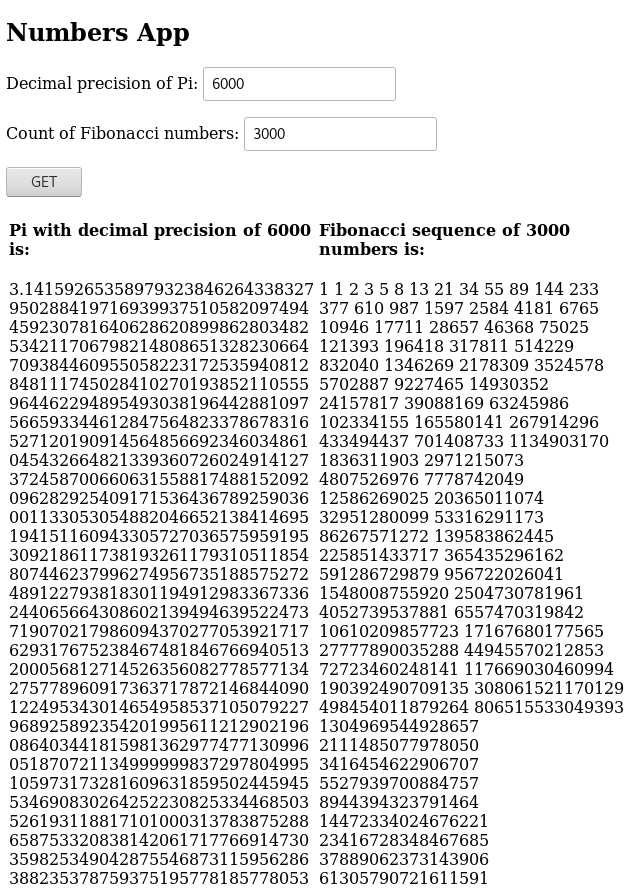
\includegraphics[width=\textwidth]{images/numbers2.png}
	\caption{Example of quickstart application}
\end{figure}

\chapter{Conclusion}

We introduced ourselves to microservice architecture, we should now have a basic understanding of its core principles, its advantages and shortcomings and its relationship to containers.

We looked into the monitoring aspect of microservices, why it is important, how it's used and different areas of monitoring. Also we presented some available open-source monitoring tools.

Then I presented my monitoring extension of SilverWare platform in form of OpenTracing Microservice Provider and Metrics Microservice Provider and examples of their usage. I finished the thesis with the demonstration of monitoring quickstart using different technologies provided by SilverWare platform.
 
All my implementations of both tracing and metrics providers and quickstart are available in the thesis attachment or in a fork of SilverWare project in my GitHub account:
\begin{itemize}
\item \textit{https://github.com/n3xtgen/SilverWare} - providers implementation in \textit{metrics-microservice-provider} and \textit{opentracing-microservice-provider} folders
\item \textit{https://github.com/n3xtgen/SilverWare-Demos} - quickstart implementation in the \textit{quickstart/monitoring} folder
\end{itemize}

After consultation with my advisor Martin Večera and incorporation of his suggestions, my work will be merged into the SilverWare master repository.

\bibliographystyle{IEEEtran}
\bibliography{sources}
\end{document}
